


\documentclass[crop,tikz]{standalone}% 'crop' is the default for v1.0, before it was 'preview'
%\usetikzlibrary{...}% tikz package already loaded by 'tikz' option
\usetikzlibrary{trees}
\usetikzlibrary{shapes}
\usetikzlibrary{trees}
\usetikzlibrary{shapes}
\usetikzlibrary{matrix, fit}
\usetikzlibrary{arrows}
\usetikzlibrary{shapes}

\usepackage{bm}

\begin{document}



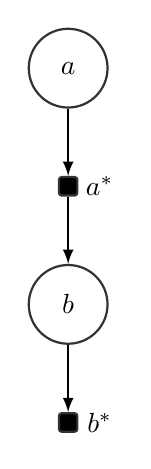
\begin{tikzpicture}

\tikzstyle{hidden}=[circle, minimum size = 10mm, thick, draw =black!80, node distance = 16mm]
\tikzstyle{observed}=[circle, minimum size = 10mm, thick, draw =black!80, node distance = 16mm, fill=gray!50]
\tikzstyle{tensor}=[rectangle, minimum size = 2mm, rounded corners=1pt, thick, draw =black!80, node distance = 16mm, fill=black]


\tikzstyle{connect}=[-latex, thick]


\node[hidden] (a) at (0,0)  {$a$};
\node[tensor] (aval) at (0,-1.5)  {$ $};
\node[] () at (0.4, -1.5)  {$a^*$};

\node[hidden] (b) at (0,-3)  {$b$};
\node[tensor] (bval) at (0,-4.5)  {$ $};
\node[] () at (0.4, -4.5)  {$b^*$};

\path (a) [connect]  edge (aval);
\path (aval) [connect]  edge (b);
\path (b) [connect]  edge (bval);







\end{tikzpicture}
\end{document}